\Opensolutionfile{ans}[ans/ansCD2D1-5]
\begin{ex}%[2D1B5-2]%Câu 1.
	Cho hàm số $y=x^3+3x^2-4$ có đồ thị $(C_1)$ và hàm số $y=-x^3+3x^2-4$ có đồ thị $(C_2)$. Khẳng định nào sau đây là đúng?
	\choice
	{$(C_1)$ và $(C_2)$ đối xứng nhau qua $Ox$}
	{$(C_1)$ và $(C_2)$ đối xứng nhau qua gốc tọa độ}
	{$(C_1)$ và $(C_2)$ trùng nhau}
	{\True $(C_1)$ và $(C_2)$ đối xứng nhau qua $Oy$}
	\loigiai{
		Xét hàm số $y=x^3+3x^2-4$ có tập xác định $\mathscr{D}=\mathbb{R}$ và $y(-x)=-x^3+3x^2-4$.\\
		Do đó $(C_1)$ và $(C_2)$ đối xứng nhau qua $Oy$.}
\end{ex}
\begin{ex}%[2D1B5-2]%Câu 2.
	Cho hàm số $y=f(x)$ có đồ thị là đường cong trong hình vẽ bên. 
	\begin{center}
		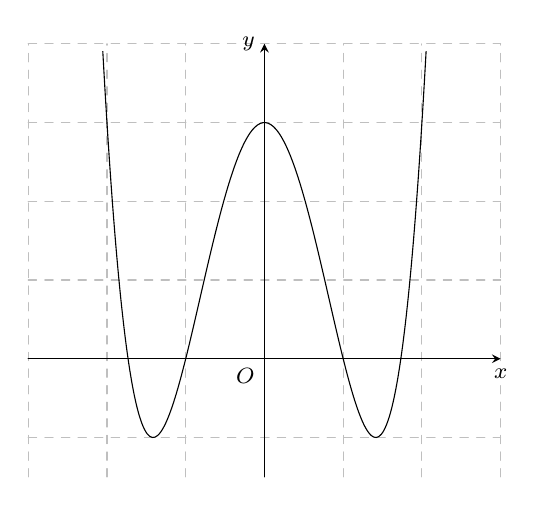
\begin{tikzpicture}[scale=1,>=stealth, font=\footnotesize, line join=round, line cap=round]
	\def\a{1} \def\b{-4} \def\c{3} % Hệ số
	\def\xmin{-3} \def\xmax{3}
	\def\ymin{-1.5} \def\ymax{4} 
	\draw[color=gray!50,dashed] (\xmin,\ymin) grid (\xmax,\ymax); 
	\draw[->] (\xmin,0)--(\xmax,0) node [below]{$x$};
	\draw[->] (0,\ymin)--(0,\ymax) node [left]{$y$};
	\node at (0,0) [below left]{$O$};
	\clip (\xmin+0.1,\ymin+0.1) rectangle (\xmax-0.5,\ymax-0.1);
	\draw[smooth,samples=300] plot(\x,{\a*(\x)^4+\b*(\x)^2+\c});
	\end{tikzpicture}
	\end{center}
	Số điểm cực trị của đồ thị hàm số $y=\left|f(x)\right|$ là
	\choice
	{$3$}
	{$5$}
	{$6$}
	{\True $7$}
	\loigiai{
		\begin{center}
			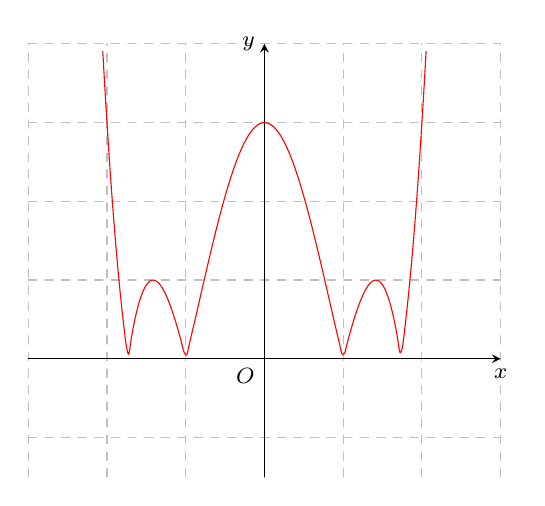
\begin{tikzpicture}[scale=1,>=stealth, font=\footnotesize, line join=round, line cap=round]
			\def\a{1} \def\b{-4} \def\c{3} % Hệ số
			\def\xmin{-3} \def\xmax{3}
			\def\ymin{-1.5} \def\ymax{4} 
			\draw[color=gray!50,dashed] (\xmin,\ymin) grid (\xmax,\ymax); 
			\draw[->] (\xmin,0)--(\xmax,0) node [below]{$x$};
			\draw[->] (0,\ymin)--(0,\ymax) node [left]{$y$};
			\node at (0,0) [below left]{$O$};
			\clip (\xmin+0.1,\ymin+0.1) rectangle (\xmax-0.5,\ymax-0.1);
			\draw[smooth,samples=300,red] plot(\x,{abs(\a*(\x)^4+\b*(\x)^2+\c)});
			\end{tikzpicture}
		\end{center}
		Dựa vào đồ thị hàm số đã cho ta có đồ thị hàm số $y=\left|f(x)\right|$\\
		Từ đó đồ thị hàm số $y=\left|f(x)\right|$ có $7$ cực trị.}
\end{ex}
\begin{ex}%[2D1B5-2]%Câu 3.
	Cho hàm số $y=f(x)$ liên tục trên $\mathbb{R}$ và có bảng biến thiên như sau
	\begin{center}
		
\begin{tikzpicture}
		\tkzTabInit[nocadre=false,lgt=1.2,espcl=2.5,deltacl=0.6]
		{$x$ /0.6, $y'$ /0.6, $y$ /2.5}
		{$-\infty$,$-2$,$0$,$+\infty$}
		\tkzTabLine{,+,$0$,-,$0$,+,}
		\tkzTabVar{-/$-\infty$,+/$5$,-/$1$,+/$+\infty$}
		\end{tikzpicture}
	\end{center}
	Đồ thị của hàm số $y=\left|f(x)\right|$ có bao nhiêu điểm cực trị?
	\choice
	{$2$}
	{\True $3$}
	{$4$}
	{$5$}
	\loigiai{
		Ta có đồ thị của hàm số $y=\left|f(x)\right|$: 
		\begin{center}
			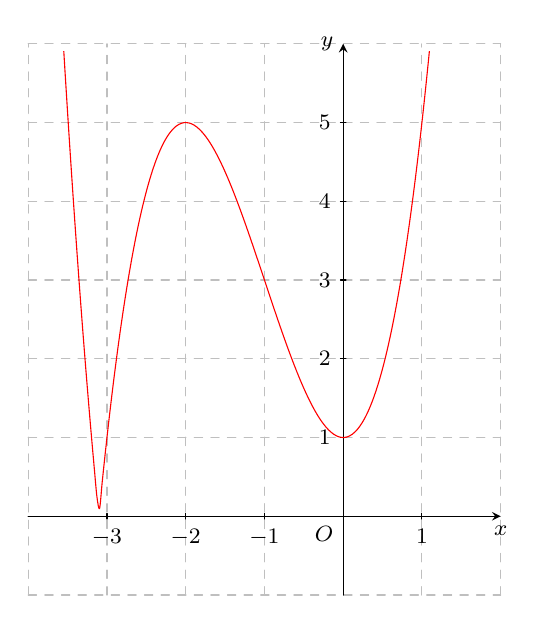
\begin{tikzpicture}[scale=1,>=stealth, font=\footnotesize, line join=round, line cap=round]
		\def\a{1} \def\b{3} \def\c{0} \def\d{1} % Hệ số
		\def\xmin{-4} \def\xmax{2}
		\def\ymin{-1} \def\ymax{6} 
		\draw[color=gray!50,dashed] (\xmin,\ymin) grid (\xmax,\ymax); 
		\draw[->] (\xmin,0)--(\xmax,0) node [below]{$x$};
		\draw[->] (0,\ymin)--(0,\ymax) node [left]{$y$};
		\node at (0,0) [below left]{$O$};
		\foreach \x in {-3,-2,-1,1}
		\draw[thin] (\x,1pt)--(\x,-1pt) node [below] {$\x$};
		\foreach \y in {1,2,...,5}
		\draw[thin] (1pt,\y)--(-1pt,\y) node [left] {$\y$};
		\clip (\xmin+0.1,\ymin+0.1) rectangle (\xmax-0.5,\ymax-0.1);
		\draw[smooth,samples=300,red] plot(\x,{abs(\a*(\x)^3+\b*(\x)^2+\c*(\x)+\d)});
		\end{tikzpicture}
		\end{center}
		Vậy đồ thị của hàm số $y=\left|f(x)\right|$ có 3 điểm cực trị.}
\end{ex}
\begin{ex}%[2D1B5-2]%Câu 4.
	Cho hàm số $y=x^3-6x^2+9x+m$ có đồ thị là $(C)$. Giả sử $(C)$ cắt trục hoành tại ba điểm có hoành độ $x_1,x_2,x_3$ (với $x_1<x_2<x_3$). Trong các khẳng định sau, khẳng định nào đúng?
	\choice
	{$x_1<0<1<x_2<3<x_3<4$}
	{$1<x_1<x_2<3<x_3<4$}
	{\True $0<x_1<1<x_2<3<x_3<4$}
	{$1<x_1<3<x_2<4<x_3$}
	\loigiai{
		Xét phương trình $x^3-6x^2+9x=-m (1)$\\
		Đồ thị của hai hàm số $\heva{&f(x)=x^3-6x^2+9x\\&g(x)=-m}$ 
		\begin{center}
			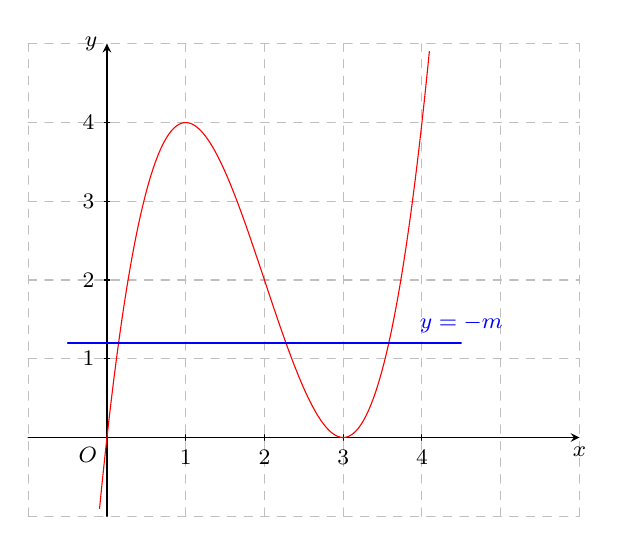
\begin{tikzpicture}[scale=1,>=stealth, font=\footnotesize, line join=round, line cap=round]
		\def\a{1} \def\b{-6} \def\c{9} \def\d{0} % Hệ số
		\def\xmin{-1} \def\xmax{6}
		\def\ymin{-1} \def\ymax{5} 
		\draw[color=gray!50,dashed] (\xmin,\ymin) grid (\xmax,\ymax); 
		\draw[->] (\xmin,0)--(\xmax,0) node [below]{$x$};
		\draw[->] (0,\ymin)--(0,\ymax) node [left]{$y$};
		\node at (0,0) [below left]{$O$};
		\foreach \x in {1,2,...,4}
		\draw[thin] (\x,1pt)--(\x,-1pt) node [below] {$\x$};
		\foreach \y in {1,2,...,4}
		\draw[thin] (1pt,\y)--(-1pt,\y) node [left] {$\y$};
		\clip (\xmin+0.1,\ymin+0.1) rectangle (\xmax-0.5,\ymax-0.1);
		\draw[smooth,samples=300,red] plot(\x,{\a*(\x)^3+\b*(\x)^2+\c*(\x)+\d});
		\draw[smooth,samples=300,blue](-0.5,1.2)--(4.5,1.2) node [above] {$y=-m$};
		\end{tikzpicture}
		\end{center}
		Để đồ thị $(C)$ cắt trục hoành tại 3 điểm phân biệt thì phương trình $(1)$ phải có 3 nghiệm phân biệt hay $0 <-m<4\Leftrightarrow-4<m<0$.\\
		Khi đó dựa vào đồ thị ta có kết quả: $0<x_1<1<x_2<3<x_3<4$.} 
\end{ex}
\begin{ex}%[2D1K5-2]%Câu 5.
	Cho hàm số $y=f(x)$ xác định trên tập $\mathbb{R}\setminus\{0\}$ và có bảng biến thiên như hình vẽ.
	\begin{center}
		
\begin{tikzpicture}
		\tikzset{double style/.append style={double distance=1.5pt}}
		\tkzTabInit[nocadre=false,lgt=1.2,espcl=2.5,deltacl=0.6]
		{$x$ /0.6,$y'$ /0.6,$y$ /2}
		{$-\infty$,$0$,$1$,$+\infty$}
		\tkzTabLine{,-,d,-,$0$,+,}
		\tkzTabVar{+/$+\infty$,-D+/$-\infty$/$+\infty$,-/$3$,+/$+\infty$}
		\end{tikzpicture}
	\end{center}
	Số nghiệm của phương trình $3\left|f(2x-1)\right|-10=0$. 
	\choice
	{\True $4$}
	{$3$}
	{$2$}
	{$1$}
	\loigiai{
		Ta có $\left|f(2x-1)\right|=\dfrac{10}{3}\Leftrightarrow\hoac{&f(2x-1)=\dfrac{10}{3}\\&f(2x-1)=-\dfrac{10}{3}.}$\\ 
		Từ bảng biến thiên của hàm số $y=f(x)$. Ta có bảng biến thiên của hàm số $y=f(2x-1)$:
		\begin{center}
			
\begin{tikzpicture}
			\tikzset{double style/.append style={double distance=1.5pt}}
			\tkzTabInit[nocadre=false,lgt=1.2,espcl=2.5,deltacl=0.6]
			{$x$ /0.6,$y'$ /0.6,$y$ /2}
			{$-\infty$,$\frac{1}{2}$,$1$,$+\infty$}
			\tkzTabLine{,-,d,-,$0$,+,}
			\tkzTabVar{+/$+\infty$,-D+/$-\infty$/$+\infty$,-/$3$,+/$+\infty$}
			\end{tikzpicture}
		\end{center}
		Phương trình $f(2x-1)=\dfrac{10}{3}$ có ba nghiệm phân biệt.\\
		Phương trình $f(2x-1)=-\dfrac{10}{3}$ có một nghiệm.\\
		Vậy phương trình đã cho có 4 nghiệm.\\
		**Giải thích rõ ràng hơn:\\
		Gọi đồ thị hàm số $y=f(x)$ là $(C)$ thì đồ thị $(C')$ của hàm số $y=f(2x-1)$ có được bằng cách co đồ thị $(C)$ về trục tung 2 lần rồi tịnh tiến sang phải 1 đơn vị nên ta có bảng biến thiên của hàm $y=f(2x-1)$ không thay đổi so với bảng biến thiên của $y=f(x)$ (mặc dù đồ thị có thay đổi về hình dạng và kích thước).}
\end{ex}
\begin{ex}%[2D1K5-2]%Câu 6.
	(THPT Chu Văn An - Hà Nội - Lần 1 - 2018) Hình vẽ dưới đây là đồ thị của hàm số $y=f(x)$.\\
	\begin{center}
		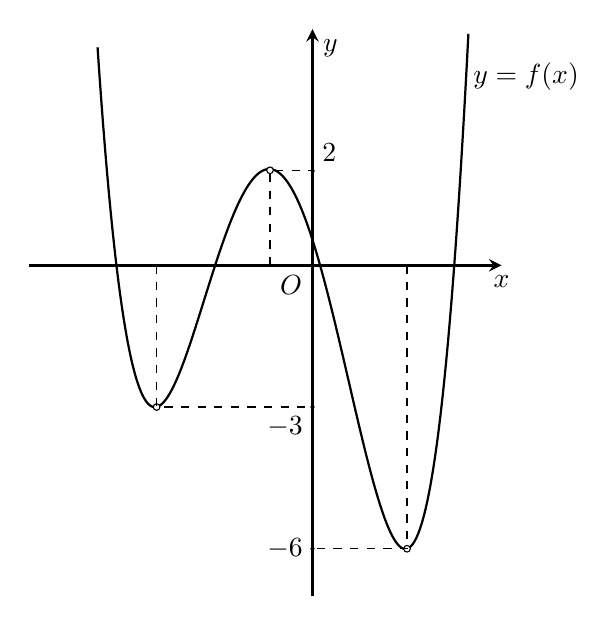
\begin{tikzpicture}[>=stealth, scale=0.6]
	\draw[->, line width = 1pt] (-6,0) -- (0,0) node[below left]{$O$} -- (4,0) node[below]{$x$};
	\draw[->, line width = 1pt] (0,-7) -- (0,0) -- (0,5) node[below right]{$y$};
	\draw[black] (3.2,3.5) node[above right]{$y=f(x)$};
	\draw[black, samples=200, thick, domain=-4.55:3.3] plot(\x,{0.13055152954432256*(\x)^(4.0)+0.3983999796654382*(\x)^(3.0)-1.3831367339901912*(\x)^(2.0)-3.1397653640733365*(\x)+0.536053354074771});
	\draw[fill=white]  (-3.3,-3) circle (2pt);
	\draw[fill=white]  (-0.9,2.011) circle (2pt);
	\draw[fill=white]  (2,-6) circle (2pt);
	\draw  (0,-6)  node[left]{$-6$}  circle (1pt);
	\draw  (0,2)  node[above right]{$2$}  circle (1pt);
	\draw  (0,-3)  node[below left]{$-3$} circle (1pt);
	\draw[dashed] (-3.3,0) -- (-3.3,-3) -- (0,-3)
	(-0.9,0) -- (-0.9,2) -- (0,2)
	(2,0) -- (2,-6) -- (0,-6);
	\end{tikzpicture}
	\end{center}
	Có bao nhiêu giá trị nguyên dương của tham số m để hàm số $y=|f(x+1)+m|$ có 5 điểm cực trị?
	\choice
	{$2$}
	{\True $3$}
	{$1$}
	{$0$}
	\loigiai{
		Đồ thị hàm số $y=f(x+1)+m$ là đồ thị hàm số $y=f(x)$ tịnh tiến sang trái 1 đơn vị và lên trên hoặc xuống dưới $|m|$ đơn vị.
		Ta có bảng biến thiên của hàm số $y=f(x+1)+m$:
		\begin{center}
			
\begin{tikzpicture}
			\tkzTabInit[nocadre=false,lgt=1.2,espcl=2.5,deltacl=0.6]
			{$x$ /0.6,$y'$ /0.6,$y$ /2}
			{$-\infty$,$-2$,$0$,$3$,$+\infty$}
			\tkzTabLine{,-,$0$,+,$0$,-,$0$,+,}
			\tkzTabVar{+/$-\infty$, -/$-3+m$,+/$2+m$,-/$-6+m$,+/$-\infty$}
			\end{tikzpicture}
		\end{center}
		Từ đó hàm số $y=|f(x+1)+m|$ có 5 cực khi khi và chỉ khi $$-6+m < 0 \leq -3+m \Rightarrow 3\leq m<6\Rightarrow m=3,4,5.$$ }
\end{ex}
\begin{ex}%[2D1K5-2]%Câu 7.
	(PTNK - Cơ sở 2 - 2018) Cho hàm số $y=f(x)=x^3-3x+2$ có bảng biến thiên như hình bên. Hàm số $y=\left|f(x)\right|$ có bảng biến thiên nào dưới đây?
	\choice
	{\True 
\begin{tikzpicture}
		\tkzTabInit[nocadre,lgt=1,espcl=2.5]
		{$x$ /.7,$y'$ /.7,$y$ /1.5}{$-\infty$,$-2$,$0$,$1$,$+\infty$}
		\tkzTabLine{,-,d,+,$0$,-,$0$,+,}
		\tkzTabVar{+/ $+\infty$ ,-/$0$,+/$4$,-/$0$,+/$+\infty$}
		\end{tikzpicture}}
	{
\begin{tikzpicture}
		\tkzTabInit[nocadre,lgt=1,espcl=2.5]
		{$x$ /.7,$y'$ /.7,$y$ /1.5}{$-\infty$,$-2$,$0$,$1$,$+\infty$}
		\tkzTabLine{,-,d,+,$0$,-,$0$,+,}
		\tkzTabVar{+/ $+\infty$ ,-/$0$,+/$2$,-/$0$,+/$+\infty$}
		\end{tikzpicture}}
	{
\begin{tikzpicture}
		\tkzTabInit[nocadre,lgt=1,espcl=2.5]
		{$x$ /.7,$y'$ /.7,$y$ /1.5}{$-\infty$,$-2$,$0$,$1$,$+\infty$}
		\tkzTabLine{,-,$0$,+,$0$,-,$0$,+,}
		\tkzTabVar{+/ $+\infty$ ,-/$0$,+/$2$,-/$0$,+/$+\infty$}
		\end{tikzpicture}}
	{
\begin{tikzpicture}
		\tkzTabInit[nocadre]{$x$/1,$y'$/1,$y$/2}{$-\infty$,$0$,$1$,$+\infty$}
		\tkzTabLine{,+,0,-,0,+,}
		\tkzTabVar{-/  $-\infty$, +/$2$,-/ $0$, +/$+\infty$ } 
		\end{tikzpicture}}
	\loigiai{
		Phương trình hoành độ giao điểm $x^3-3x+2=0\Leftrightarrow\hoac{&x=1\\&x=-2.}$ \\
		Đồ thị hàm số $y=\left|f(x)\right|$ được vẽ như sau:\\
		+ Giữ nguyên đồ thị hàm số $y=f(x)=x^3-3x+2$ phần nằm trên trục $Ox$.\\
		+ Lấy đối xứng qua trục $Ox$ phần đồ thị $y=f(x)=x^3-3x+2$ phía dưới trục $Ox$.\\
		Do đó hàm số $y=\left|f(x)\right|$ có bảng biến thiên là A.}
\end{ex}
\begin{ex}%[2D1K5-2]%Câu 8.
	Tìm số nghiệm thực của phương trình $2|x|^3-9x^2+12|x|-\dfrac{9}{2}=0$. 
	\choice
	{$4$}
	{$2$}
	{\True $6$}
	{$3$}
	\loigiai{
		\begin{center}
			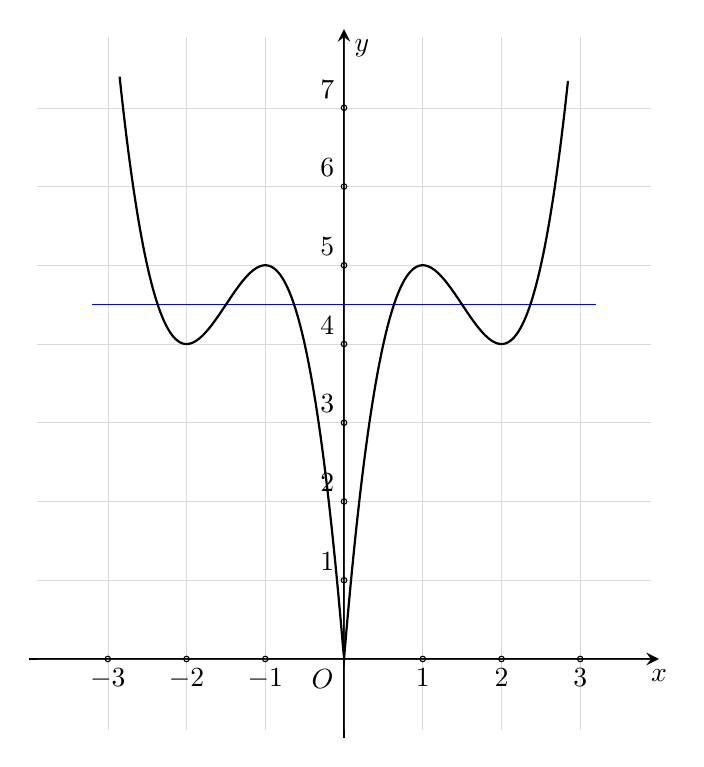
\begin{tikzpicture}[>=stealth, scale=1]
		\draw[->, line width = 1pt] (-4,0) -- (0,0) node[below left]{$O$} -- (4,0) node[below]{$x$};
		\draw[->, line width = 1pt] (0,-1) -- (0,0) -- (0,8) node[below right]{$y$};
		\draw[step=1cm,gray,opacity=.3,very thin] (-3.9,-0.9) grid (3.9,7.9);
		\draw[blue] (-3.2,4.5) -- (3.2,4.5);
		\draw[ samples=600, thick, domain=-2.85:2.85] plot(\x,{2.0*abs((\x))^(3.0)-9.0*(\x)^(2.0)+12.0*abs((\x))});
		\draw  (-1,0)  node[below]{$-1$}  circle (1pt);
		\draw  (-2,0)  node[below]{$-2$}  circle (1pt);
		\draw  (-3,0)  node[below]{$-3$}  circle (1pt);
		\draw  (1,0)  node[below]{$1$}  circle (1pt);
		\draw  (2,0)  node[below]{$2$}  circle (1pt);
		\draw  (3,0)  node[below]{$3$}  circle (1pt);
		\draw  (0,7)  node[above left]{$7$}  circle (1pt);
		\draw  (0,6)  node[above left]{$6$}  circle (1pt);
		\draw  (0,5)  node[above left]{$5$}  circle (1pt);
		\draw  (0,4)  node[above left]{$4$}  circle (1pt);
		\draw  (0,3)  node[above left]{$3$}  circle (1pt);
		\draw  (0,2)  node[above left]{$2$}  circle (1pt);
		\draw  (0,1)  node[above left]{$1$}  circle (1pt);
		\end{tikzpicture}
		\end{center}
		$2|x|^3-9x^2+12|x|-\dfrac{9}{2}=0(1)\Leftrightarrow 2|x|^3-9x^2+12|x|=\dfrac{9}{2}\quad(*)$.\\
		Phương trình $(*)$ là phương trình hoành độ giao điểm của $\heva{&y=2|x|^3-9x^2+12|x|\quad(C)\\&y=\dfrac{9}{2}.\quad(d)}$ \\
		Số nghiệm phương trình $(1)$ là số giao điểm của $(C)$ và $(d)$.\\
		Dựa vào đồ thị ta thấy phương trình $(1)$ có $6$ nghiệm.}
\end{ex}
\begin{ex}%[2D1G5-2]%Câu 9.
	Cho hàm số $y=f(x)$ có đạo hàm trên $\mathbb{R}$ và có đồ thị như hình vẽ. 
	\begin{center}
		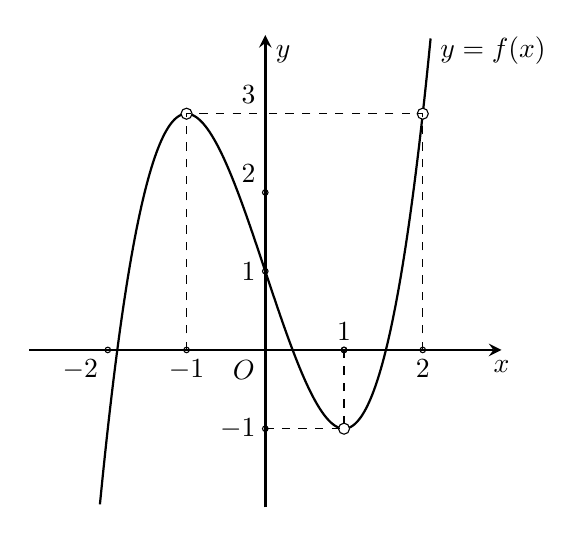
\begin{tikzpicture}[>=stealth, scale=1]
	\draw[->, line width = 1pt] (-3,0) -- (0,0) node[below left]{$O$} -- (3,0) node[below]{$x$};
	\draw[->, line width = 1pt] (0,-2) -- (0,0) -- (0,4) node[below right]{$y$};
	\draw[black] (2.1,3.5) node[above right]{$y=f(x)$};
	\draw[black, samples=200, thick, domain=-2.1:2.1] plot(\x,{(\x)^(3.0)-3.0*(\x)+1.0});
	\draw  (-1,0)  node[below]{$-1$}  circle (1pt);
	\draw  (-2,0)  node[below left]{$-2$}  circle (1pt);
	\draw  (1,0)  node[above]{$1$}  circle (1pt);
	\draw  (0,1)  node[left]{$1$}  circle (1pt);
	\draw  (2,0)  node[below]{$2$}  circle (1pt);
	\draw[fill=white]  (-1,3) circle (2pt);
	\draw[fill=white]  (1,-1) circle (2pt);
	\draw[fill=white]  (2,3) circle (2pt);
	\draw  (0,-1)  node[left]{$-1$}  circle (1pt);
	\draw  (1,0)  circle (1pt);
	\draw  (0,2)  node[above left]{$2$}  circle (1pt);
	\draw  (0,3)  node[above left]{$3$};
	\draw[dashed] (-1,0) -- (-1,3) -- (0,3)
	(0,-1) -- (1,-1) -- (1,0)
	(2,0) -- (2,3) -- (0,3);
	\end{tikzpicture}
	\end{center}
	Đặt hàm số $y=g(x)=f\left(2x^3+x-1\right)+m$. Tìm $m$ để $\max\limits_{[0; 1]} g(x)=-10$. 
	\choice
	{\True $m=-13$}
	{$m=3$}
	{$m=-12$}
	{$m=-1$}
	\loigiai{
		$\max\limits_{[0; 1]} g(x)=\max\limits_{[-1; 2]} f(x)+m=3+m$ \\
		$ \Rightarrow 3+m=-10\Leftrightarrow m=-13 $.}
\end{ex}
\begin{ex}%[2D1G5-2]%Câu 10.
	Hình vẽ dưới là đồ thị của hàm số $y=f(x)$.
	\begin{center}
		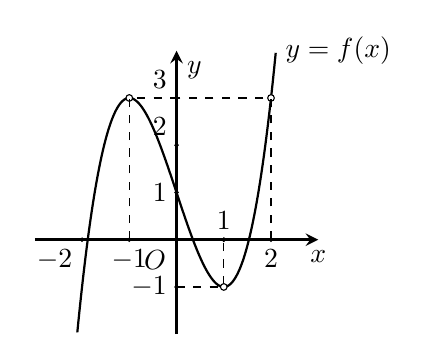
\begin{tikzpicture}[>=stealth, scale=0.6]
		\draw[->, line width = 1pt] (-3,0) -- (0,0) node[below left]{$O$} -- (3,0) node[below]{$x$};
		\draw[->, line width = 1pt] (0,-2) -- (0,0) -- (0,4) node[below right]{$y$};
		\draw[black] (2.1,3.5) node[above right]{$y=f(x)$};
		\draw[black, samples=200, thick, domain=-2.1:2.1] plot(\x,{(\x)^(3.0)-3.0*(\x)+1.0});
		\draw  (-1,0)  node[below]{$-1$}  circle (1pt);
		\draw  (-2,0)  node[below left]{$-2$}  circle (1pt);
		\draw  (1,0)  node[above]{$1$}  circle (1pt);
		\draw  (0,1)  node[left]{$1$}  circle (1pt);
		\draw  (2,0)  node[below]{$2$}  circle (1pt);
		\draw[fill=white]  (-1,3) circle (2pt);
		\draw[fill=white]  (1,-1) circle (2pt);
		\draw[fill=white]  (2,3) circle (2pt);
		\draw  (0,-1)  node[left]{$-1$}  circle (1pt);
		\draw  (1,0)  circle (1pt);
		\draw  (0,2)  node[above left]{$2$}  circle (1pt);
		\draw  (0,3)  node[above left]{$3$};
		\draw[dashed] (-1,0) -- (-1,3) -- (0,3)
		(0,-1) -- (1,-1) -- (1,0)
		(2,0) -- (2,3) -- (0,3);
		\end{tikzpicture}
	\end{center}
	 Gọi $S$ là tập hợp các giá trị nguyên dương của tham số $m$ để đồ thị hàm số $y=\left|f(x-2)+m\right|$ có $5$ điểm cực trị. Tổng giá trị tất cả các phần tử của $S$ bằng
	\choice
	{$15$}
	{$18$}
	{$9$}
	{\True $12$}
	\loigiai{
		\begin{center}
			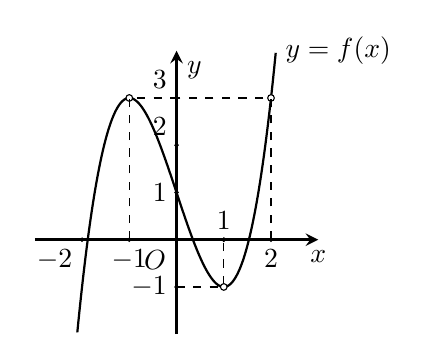
\begin{tikzpicture}[>=stealth, scale=0.6]
		\draw[->, line width = 1pt] (-3,0) -- (0,0) node[below left]{$O$} -- (3,0) node[below]{$x$};
		\draw[->, line width = 1pt] (0,-2) -- (0,0) -- (0,4) node[below right]{$y$};
		\draw[black] (2.1,3.5) node[above right]{$y=f(x)$};
		\draw[black, samples=200, thick, domain=-2.1:2.1] plot(\x,{(\x)^(3.0)-3.0*(\x)+1.0});
		\draw  (-1,0)  node[below]{$-1$}  circle (1pt);
		\draw  (-2,0)  node[below left]{$-2$}  circle (1pt);
		\draw  (1,0)  node[above]{$1$}  circle (1pt);
		\draw  (0,1)  node[left]{$1$}  circle (1pt);
		\draw  (2,0)  node[below]{$2$}  circle (1pt);
		\draw[fill=white]  (-1,3) circle (2pt);
		\draw[fill=white]  (1,-1) circle (2pt);
		\draw[fill=white]  (2,3) circle (2pt);
		\draw  (0,-1)  node[left]{$-1$}  circle (1pt);
		\draw  (1,0)  circle (1pt);
		\draw  (0,2)  node[above left]{$2$}  circle (1pt);
		\draw  (0,3)  node[above left]{$3$};
		\draw[dashed] (-1,0) -- (-1,3) -- (0,3)
		(0,-1) -- (1,-1) -- (1,0)
		(2,0) -- (2,3) -- (0,3);
		\end{tikzpicture}
		\end{center}
		Cách 1: dùng đồ thị.\\
		- Nhận thấy: số giao điểm của $(C)\colon y=f(x)$ với $Ox$ bằng số giao điểm của $(C_1)\colon y=f(x-2)$ với $Ox$.\\
		Vì $m>0$ nên $(C_2)\colon y=f(x-2)+m$ có được bằng cách tịnh tiến $(C_1)\colon y=f(x-2)$ lên trên $m$ đơn vị.\\
		- Đồ thị hàm số $y=\left|f(x-2)+m\right|$ có được bằng cách lấy đối xứng qua trục hoành $Ox$ phần đồ thị $(C_2)$ nằm phía dưới trục $Ox$ và giữ nguyên phần phía trên trục $Ox$.\\
		- Ta xét các trường hợp sau:\\ 
		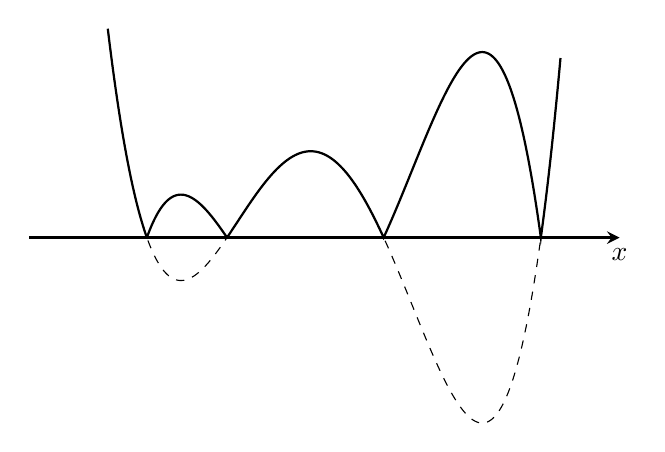
\begin{tikzpicture}[>=stealth, scale=0.5]
		\draw[->, line width = 1pt] (-6,0) -- (0,0) -- (9,0) node[below]{$x$};
		\draw[black, samples=500, dashed, domain=-4:7.5] plot(\x,{0.02288943232705914*(\x)^(4.0)-0.1379588795620629*(\x)^(3.0)-0.36270849882733597*(\x)^(2.0)+1.2474337172745027*(\x)+1.4077858321786338});
		\draw[black, samples=600, thick, domain=-4:7.5]
		plot(\x,{abs(0.02288943232705914*(\x)^(4.0)-0.1379588795620629*(\x)^(3.0)-0.36270849882733597*(\x)^(2.0)+1.2474337172745027*(\x)+1.4077858321786338)});
		\end{tikzpicture}
		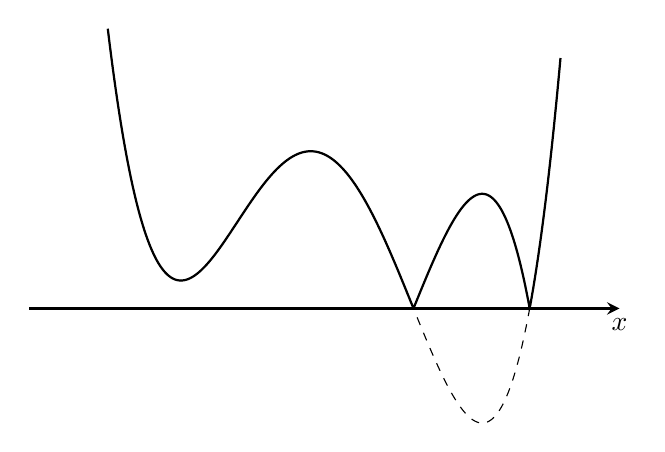
\begin{tikzpicture}[>=stealth, scale=0.5]
		\draw[->, line width = 1pt] (-6,0) -- (0,0) -- (9,0) node[below]{$x$};
		\draw[black, samples=500, dashed, domain=-4:7.5] plot(\x,{0.02288943232705914*(\x)^(4.0)-0.1379588795620629*(\x)^(3.0)-0.36270849882733597*(\x)^(2.0)+1.2474337172745027*(\x)+1.4077858321786338+1.8});
		\draw[black, samples=600, thick, domain=-4:7.5]
		plot(\x,{abs(0.02288943232705914*(\x)^(4.0)-0.1379588795620629*(\x)^(3.0)-0.36270849882733597*(\x)^(2.0)+1.2474337172745027*(\x)+1.4077858321786338+1.8)});
		\end{tikzpicture}\\
		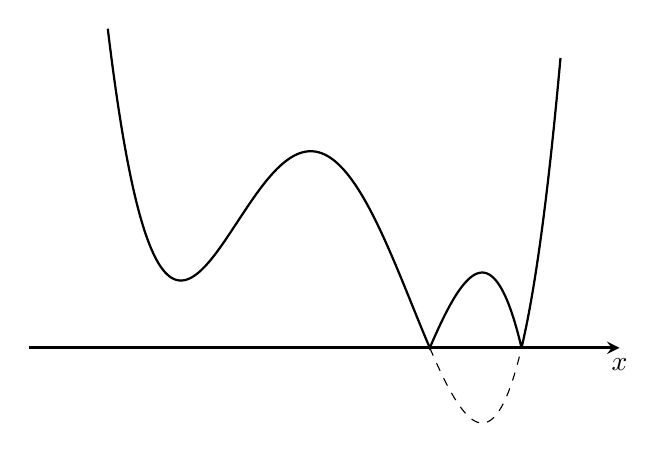
\begin{tikzpicture}[>=stealth, scale=0.5]
		\draw[->, line width = 1pt] (-6,0) -- (0,0) -- (9,0) node[below]{$x$};
		\draw[black, samples=500, dashed, domain=-4:7.5] plot(\x,{0.02288943232705914*(\x)^(4.0)-0.1379588795620629*(\x)^(3.0)-0.36270849882733597*(\x)^(2.0)+1.2474337172745027*(\x)+1.4077858321786338+2.8});
		\draw[black, samples=600, thick, domain=-4:7.5]
		plot(\x,{abs(0.02288943232705914*(\x)^(4.0)-0.1379588795620629*(\x)^(3.0)-0.36270849882733597*(\x)^(2.0)+1.2474337172745027*(\x)+1.4077858321786338+2.8)});
		\end{tikzpicture}
		\begin{tikzpicture}[>=stealth, scale=0.5]
		\draw[->, line width = 1pt] (-6,0) -- (0,0) -- (9,0) node[below]{$x$};
		\draw[black, samples=500, dashed, domain=-4:7.5] plot(\x,{0.02288943232705914*(\x)^(4.0)-0.1379588795620629*(\x)^(3.0)-0.36270849882733597*(\x)^(2.0)+1.2474337172745027*(\x)+1.4077858321786338+4.7});
		\draw[black, samples=600, thick, domain=-4:7.5]
		plot(\x,{abs(0.02288943232705914*(\x)^(4.0)-0.1379588795620629*(\x)^(3.0)-0.36270849882733597*(\x)^(2.0)+1.2474337172745027*(\x)+1.4077858321786338+4.7)});
		\end{tikzpicture}\\
		+ Trường hợp 1: $0<m<3$: đồ thị hàm số có 7 điểm cực trị (loại).\\
		+ Trường hợp 2: $m=3$: đồ thị hàm số có 5 điểm cực trị (thỏa mãn).\\
		+ Trường hợp 3: $3<m<6$: đồ thị hàm số có 5 điểm cực trị (thỏa mãn).\\
		+ Trường hợp 4: $m\geq 6$: đồ thị hàm số có 3 điểm cực trị (loại).\\
		Vậy $3\leq m<6$ Do $m\in\mathbb{Z}_+^{*}$ nên $m\in\{3;4;5\}$ hay $S=\{3;4;5\}$.\\
		Vậy tổng giá trị tất cả các phần tử của $S$ bằng $12$.\\
		* Cách 2: đạo hàm hàm số hợp.\\
		- Ta có: $y=\left|f(x-2)+m\right|=\sqrt{[f(x-2)+m]^2}\Rightarrow y'=\dfrac{\left(f(x-2)+m\right)\cdot f'(x-2)}{\sqrt{[f(x-2)+m]^2}}$.\\
		- Xét $f'(x-2)=0 (1)$.\\
		+ Do phương trình $f'(x)=0$ có $3$ nghiệm phân biệt nên phương trình $f'(x-2)=0$ cũng có $3$ nghiệm phân biệt.\\
		- Xét $f(x-2)+m=0\Leftrightarrow f(x-2)=-m (2)$.\\
		+ Nếu $-6 <-m <-3\Leftrightarrow 3<m<6$ thì phương trình $(2)$ có $2$ nghiệm phân biệt khác $3$ nghiệm của $(1)$.\\
		+ Nếu $-m=-3\Leftrightarrow m=3$ thì $(2)$ có $3$ nghiệm phân biệt (trong đó có $2$ nghiệm đơn khác $3$ nghiệm của $(1)$ và $1$ nghiệm kép trùng với $1$ nghiệm của $(1)$).\\
		Tóm lại: với $3\leq m<6$ thì hai phương trình $(1)$ và $(2)$ có tất cả $5$ nghiệm bội lẻ phân biệt và $y'$ đổi dấu khi $x$ đi qua các nghiệm đó, hay đồ thị hàm số $y=\left|f(x-2)+m\right|$ có $5$ điểm cực trị.\\
		- Lại do $m\in\mathbb{Z}_+^{*}$ nên $m\in\{3;4;5\}$ hay $S=\{3;4;5\}$.\\
		Vậy tổng giá trị tất cả các phần tử của $S$ bằng $12$.}
\end{ex}
\begin{ex}%[2D1G5-2]%Câu 11.
	Cho hàm số $y=f(x)$ xác định trên $\mathbb{R}$ và có bảng biến thiên như hình vẽ sau: 
	\begin{center}
		
\begin{tikzpicture}
	\tkzTabInit[nocadre]{$x$/1,$y'$/1,$y$/2}{$-\infty$,$1$,$2$,$+\infty$}
	\tkzTabLine{,+,0,-,0,+,}
	\tkzTabVar{-/  $-\infty$, +/$0$,-/ $-1$, +/$+\infty$ } 
	\end{tikzpicture}
	\end{center}
	Tìm tất cả các giá trị của tham số $m$ để đồ thị của hàm số $y=\left|f(|x|)+m\right|$ có $11$ điểm cực trị. 
	\choice
	{$m\geq 0$}
	{$m\leq 0$}
	{$0\leq m\leq 1$}
	{\True $0<m<1$}
	\loigiai{
		Ta có bảng biến thiên của hàm số $y=f(|x|)+m$: 
		\begin{center}
			
\begin{tikzpicture}
		\tkzTabInit[nocadre,lgt=1,espcl=2]{$x$/1,$y'$/1,$y$/2.5}{$-\infty$,$-2$,$-1$,$0$,$1$,$2$,$+\infty$}
		\tkzTabLine{,-,0,+,0,-,d,+,0,-,0,+,}
		\tkzTabVar{+/  $+\infty$, -/$m-1$,+/ $m$, -/$m+a$,+/$m$,-/$m-1$,+/$+\infty$} 
		\end{tikzpicture}
		\end{center}
		Để đồ thị của hàm số $y=\left|f(|x|)+m\right|$ có $11$ điểm cực trị thì $\heva{&m>0\\&m-1<0}\Leftrightarrow 0<m<1$.}
\end{ex}
\begin{ex}%[2D1G5-2]%Câu 12.
	Cho hàm số $y=f(x)$ liên tục trên R có đồ thị như hình vẽ. Có bao nhiêu giá trị nguyên của m để phương trình $f(6\sin x+8\cos x)=f(m(m+1))$ có nghiệm $x\in \mathbb{R}$. 
	\begin{center}
		\begin{tikzpicture}[>=stealth, scale=1]
	\draw[->, line width = 1pt] (-3,0) -- (0,0) node[below right]{$O$} -- (3,0) node[below]{$x$};
	\draw[->, line width = 1pt] (0,-3) -- (0,0) -- (0,5) node[below right]{$y$};
	\draw[black, samples=200, thick, domain=-1.55:1.55] plot(\x,{(\x)^3+1});
	\draw  (-1,0)  node[below right]{$-1$}  circle (1pt);
	\draw  (-2,0)  node[below]{$-2$}  circle (1pt);
	%\draw  (-3,0)  node[below]{$-3$}  circle (1pt);	
	\draw  (1,0)  node[below]{$1$}  circle (1pt);
	\draw  (2,0)  node[below]{$2$}  circle (1pt);
	%\draw  (3,0)  node[below]{$3$}  circle (1pt);
	\draw  (0,4)  node[above left]{$4$}  circle (1pt);
	\draw  (0,3)  node[above left]{$3$}  circle (1pt);
	\draw  (0,2)  node[above left]{$2$}  circle (1pt);
	\draw  (0,1)  node[above left]{$1$}  circle (1pt);
	\end{tikzpicture}
	\end{center}
	\choice
	{$5$}
	{$2$}
	{4}
	{\True 6}
	\loigiai{
		Dựa vào đồ thị $y=f(x)$ là hàm số đồng biến trên R.\\
		Ta có $f(6\sin x+8\cos x)=f(m(m+1))\Leftrightarrow 6\sin x+8\cos x=m(m+1)$ \\
		$ \Leftrightarrow 10\sin (x+\alpha)=m(m+1) $,(trong đó $cos\alpha=\dfrac{3}{5}$).\\
		Phương trình có nghiệm $x\in \mathbb{R}$. $\Leftrightarrow-10\leq m(m+1)\leq 10$.\\
		Vì $m$ nguyên nên $m\in\left\{-3;-2;-1;0;1;2\right\}$.}
\end{ex}
\Closesolutionfile{ans}	
